\documentclass[a4paper, 10pt]{article}
\usepackage{fullpage} % changes the margin
\usepackage[english]{babel}
\usepackage[utf8]{inputenc}
\usepackage{hyperref}
\usepackage{xcolor}
\usepackage{graphicx}
\usepackage{array}
\usepackage{float}
\usepackage{longtable}
\usepackage[bottom]{footmisc}
\usepackage{cite}
\usepackage{parskip}
\usepackage{subcaption}
\usepackage{amssymb}
\usepackage{amsmath}
\usepackage{listings}

\hypersetup{
	colorlinks=true,       % false: boxed links; true: colored links
	linkcolor=blue,        % color of internal links
	citecolor=blue,        % color of links to bibliography
	filecolor=magenta,     % color of file links
	urlcolor=blue
}

% TEMPLATE SETTINGS
\setlength{\parindent}{0cm}
\setlength{\parskip}{2mm}
\renewcommand{\baselinestretch}{1.2}

%\setlength{\parindent}{0cm}
\newcommand{\code}[1]{\texttt{#1}}
\renewcommand{\arraystretch}{1.2}

\graphicspath{{../plots/}}

\begin{document}

\noindent
\begin{flushright}
	\large\textbf{Miguel Alcón Doganoc} \\
	Multiprocessors Architecture \\
	%\today
	June 29, 2020
\end{flushright}
\vspace{10mm}
\noindent
{\huge{\textbf{State-of-the-art in the design and certification process of Autonomous Driving systems}}}
\section{Introduction}
In the past few years, there have been lots of research and development in both industry and academia about the design and certification of Autonomous Driving (AD) systems. Safety-critical systems are typically control systems whose design and verification is data-independent, and data is mostly used for validation in the form of tests. However, AD systems, which are safety-critical real-time systems, increasingly build on deep learning, whose implementation relies on systems designed together with training data sets, thus making data (including training dataset for deep learning models) part of the design and verification phase, which is against the design and verification principles in safety standards. Recently, there has been some research activity in this direction, trying to fill the gap between the emerging challenges that the complexity of AD systems impose on their design and certification process. In this work, I give some insights on the latest research about this topic.

%Our objective in this project is to study the latest research and provide a survey of the most promising works that have been done.

\section{Challenges in Autonomous Vehicle Testing and Validation~\cite{challenges}}
The development process of safety-related automotive systems is well-defined in the ISO 26262~\cite{ISO26262}, the main functional safety standard for road vehicles. The ISO 26262 development V process (see Figure~\ref{fig:v}) sets up a framework that ties each type of testing to a corresponding design or requirement document. It represents a methodical process of creation followed by verification and validation. The left side of the V works its way from requirements through design to implementation. Instead, its right side iteratively verifies and validates larger and larger chunks of the system as it climbs back up from small components to a system-level assessment. 
\begin{figure}[htbp]
	\centering
	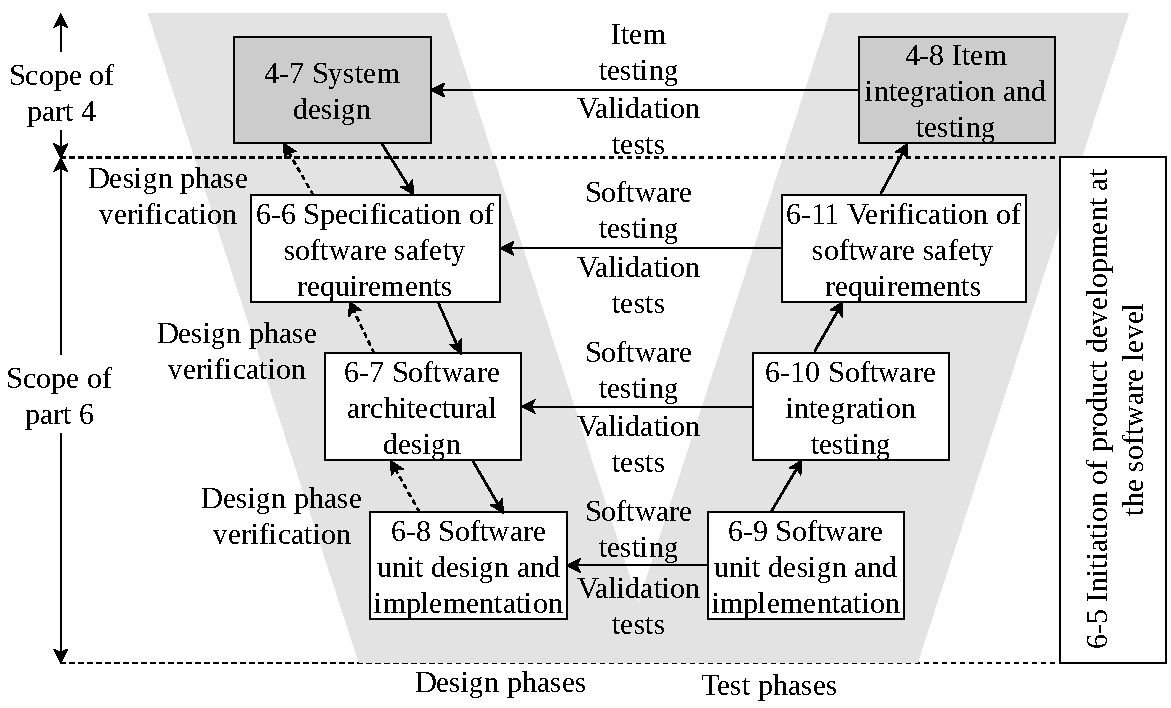
\includegraphics[width=0.8\linewidth]{figures/Part6development.pdf}
	\caption{The ISO 26262 development V process (picture taken from ISO 26262 Part 6~\cite{ISO26262}).}
	\label{fig:v}
\end{figure}

The problem here is that ISO 26262 presents challenges when adapted to deal with the sorts of novel testing issues that face autonomous vehicles (AV), and AVs cannot be considered safe unless and until they are shown to conform or map to ISO 26262 or some other suitable, widely accepted software safety standard. For this reason, the paper discussed in this section identifies five major challenge areas in testing according to the V model for AVs: driver out of the loop, complex requirements, non-deterministic algorithms, inductive learning algorithms, and fail-operational systems. The paper also identifies the general solution approaches that seem promising across these different challenge areas: phased deployment using successively relaxed operational scenarios, use of a monitor/actuator pair architecture to separate the most complex autonomy functions from simpler safety functions, and fault injection as a way to perform more efficient edge case testing.

\subsection{Driver Out of the Loop}
The hardest challenge in a fully AV is dealing with the fact that the driver is no longer driving the vehicle, which means that the driver cannot be counted on to provide control inputs to the vehicle during operation. This is a tough challenge since typical automotive safety arguments for low-integrity devices hinge upon the ability of a human driver to exert control. For instance, with an Advanced Driver Assistance System (ADAS), if a software fault causes a potentially dangerous situation, the driver might be expected to over-ride that software function and recover to a safe state. Situations in which the driver does not have an ability to take corrective action are said to lack controllability, and thus must be designed to a higher Automotive Safety Integrity Level (ASIL). Each element of an AV is attached to an ASIL, which specifies the element's necessary safety requirements for achieving an acceptable residual risk. The ASIL ranges from A to D, where D is the most stringent safety level and A the least.

One way to handle a potentially high-ASIL autonomy function is to use ASIL decomposition via a combination of a monitor/actuator architecture and redundancy. In a monitor/actuator architecture, the primary functions are performed by one module (the actuator), and a paired module (the monitor) performs an acceptance test or validation to the results of the first, thus checking the correct behaviour of the actuator. If the actuator misbehaves, the monitor shuts both modules down, resulting in a fail-silent system (i.e., any failure results in a silent component). If the monitor/actuator pair is designed correctly, the actuator can be designed to a low ASIL whether the monitor has a sufficiently high ASIL and detects all possible faults in the monitor. However, this kind of architecture causes loss of the actuator function if something goes wrong, which is a problem for a function that cannot fail operationally, such as steering in a moving vehicle. Hence, once the system detects that some of the autonomy functions are not working properly, it must somehow bring itself to a safe state.

\subsection{Complex Requirements}
As explained before, removing the driver from the control system implies that the system itself has to handle exceptions. These exceptions can be the consequence of different situations, such as bad weather, traffic rule violations, local driving conventions, or animal hazards. Even each of these situations can happen simultaneously. The challenge presented here is that the system's requirements should be clear about what is within the scope of its design, as well as what is not. However, AVs have simply too many requirements to enumerate in a classical written requirements specification. Thus, it seems unlikely that a classical V process that starts with a document that enumerates all system requirements will be scalable to AV exception handling in a rigorous way, at least in the immediate future.

One way to manage the complexity of requirements is to constrain operational concepts and engage in a phased expansion of requirements. For instance, limiting operational concepts to specific road access, visibility, vehicular environment, external environment, or speed. This is already being done by developers who might concentrate on-road testing in particular geographic regions, thus limiting the the weather the AV can be exposed to and the roads or highways it can navigate on, which determines the speed limit too.

Once sufficient confidence is gained regarding the requirements for a particular operational concept, additional similar operational concepts can be added over time to expand the envelope of allowable automation scenarios. This will not entirely eliminate the issue of complex requirements, but it can help mitigate the combinatorial explosion of requirements and exceptions that would otherwise occur.

\subsection{Non-Deterministic and Statistical Algorithms}
Some of the technologies used in AVs are inherently statistical in nature. In general, they tend to be non-deterministic, giving answers that are only correct to some probability. Validating such systems presents challenges not typically found in traditional automotive control systems. One possible problem to face when performing a vehicle-level test is the fact that, in the same scenario, the process under evaluation could potentially lead to a different outcome despite attempts to exercise nominally identical test cases. Moreover, classification algorithms (e.g., selecting the type of obstacle the AV is facing, such as pedestrians, cars or cyclists), which are non-deterministic, exhibit a tradeoff between false negatives and false positives, with fewer of one necessarily incurring more of the other. The testing implications of this are that the results of these algorithms can be incorrect and, depending on construction, they might report a particular situation as being true when there is only a moderately high probability of that situation actually being true.
%, and they can ne very sensitive to small changes in the initial conditions.

Handling non-determinism in testing is difficult for at least two reasons. The first is that it can be challenging to exercise a particular specific edge-case situation. This can occur because the system might behave in a way that activates an edge case only if it receives a very specific sequence of inputs from the world, which could be hard due to factors discussed earlier. The second is that it can be tough to evaluate whether test results are correct or not, because there is no unique correct system behaviour for a given test case. For this reason, testing non-deterministic algorithms is likely to take a a lot of more tests than simple functional validation, especially if the behaviour in question is safety-critical and expected to have an extremely low failure rate.

%Probabilistic system behaviors present a similar challenge to validation, because passing a test once does not mean that the test will be passed every time. Therefore, testing might not be oriented toward determining if behaviors are correct, but rather to validating that the statistical characteristics of the behaviour are accurately specified.

\subsection{Machine Learning Systems}

\section{Autonomous Vehicles Testing Methods Review~\cite{methods}}


\bibliographystyle{unsrt}
\bibliography{cite}


\end{document}